\documentclass[../sk-egzamin.tex]{subfiles}

\begin{document}

\question{
Co to jest segment TCP? Jakie pola zawiera nagłówek segmentu TCP?
}

\subsection*{Segment TCP}
\textbf{Segment TCP} to porcja danych utworzona przez oprogramowanie
implementujące protokół TCP w \textbf{warstwie transportu} \parit{czwartej}.
Zawiera w sobie komunikat
\parit{porcję danych utworzoną w warstwie aplikacji}.

\subsection*{Nagłówek TCP}

\begin{center}
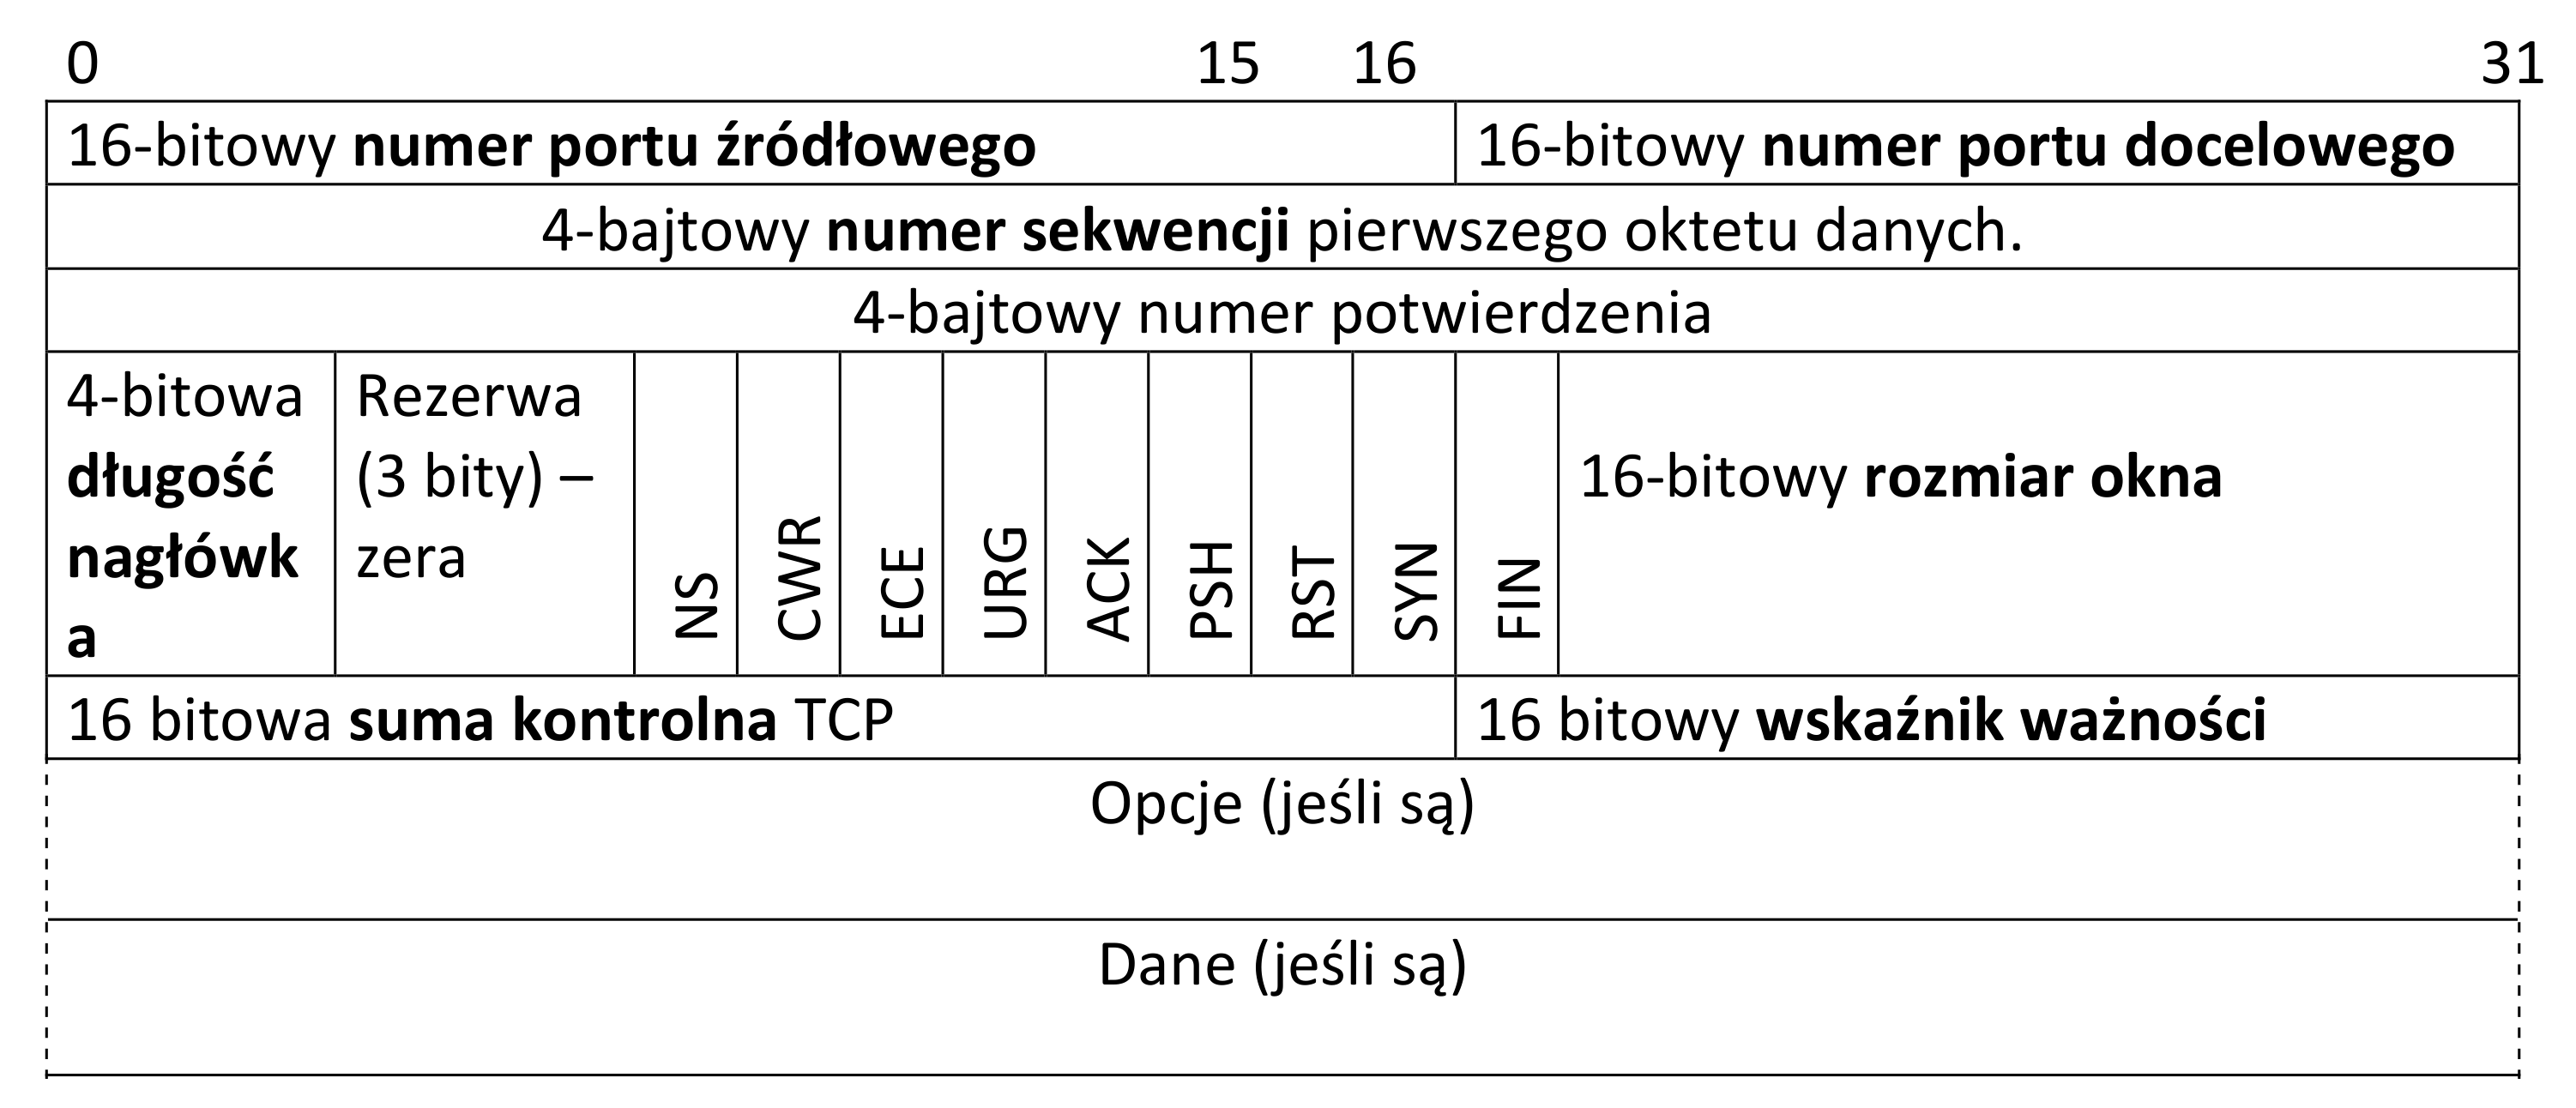
\includegraphics[width=\textwidth]{tcp-segment}
\end{center}

\begin{itemize}
    \item \textbf{Numer sekwencji}
    \begin{itemize}
        \item Dla segmentu z ustawionym tylko \texttt{SYN} wpisywany jest
        numer sekwencji początkowej \parit{ISN - Initial Seqience Number}.
        \item Wysyłany w celu rozpoczęcia nawiązywania połączenia.
        \item Pierwszy oktet danych będzie miał numer \texttt{ISN + 1}.
    \end{itemize}
    \item \textbf{Numer potwiedzenia}
    \begin{itemize}
        \item Ważny tylko przy włączonym \texttt{ACK}.
        \item Gdy segment zawiera potwierdzenie odebrania jakiegoś segmentu.
        \item To kolejny numer bajta, którego spodziewa się wysyłający
        potwierdzenie.
    \end{itemize}
    \item \textbf{Długość nagłówka} \parit{przesunięcie danych}
    \item \textbf{Flagi}
    % \begin{itemize}
    %     \item \texttt{NS, CWR, ECE} - związane z przeciwdziałaniem przeciążeniom
    %     na routerach.
    %     \item \texttt{NS} \parit{Nonce Sum}
    %     \item \texttt{CWR}
    %     \item \texttt{ECE}
    %     \item \texttt{URG}
    %     \item \texttt{ACK}
    %     \item \texttt{PSH}
    %     \item \texttt{RST}
    %     \item \texttt{SYN}
    %     \item \texttt{FIN}
    % \end{itemize}
    \item \textbf{Rozmiar okna} - liczba bajtów, które odbiorca może
    zaakceptować.
    \item \textbf{Suma kontrolna} - liczona dla nagłowka i danych z użyciem
    \textit{pseudonagłówka}, analogicznie jak w UDP oraz IP.
    \item \textbf{Wskaźnik ważności}
    \begin{itemize}
        \item Brane pod uwagę tylko jeśli bit \texttt{URG} jest ustawiony.
        \item Dodatnie przesuniecie, które musi być dodane do numeru
        przesunięcia sekwencyjnego pierwszego oktetu danych aby uzyskać numer
        ostatniego bajta szczególnie ważnych danych w segmencie.
    \end{itemize}
    \item \textbf{Opcje}
    \begin{itemize}
        \item Rodzaj opcji \parit{bajt}, długość opcji \parit{bajt}, opcja.
        \item Najważniejsza - \texttt{MSS} - \textbf{Maximum Segment Size}.
        \begin{itemize}
            \item Może być uzyskana jako \textit{Maximum Transmission Unit}
            minus rozmiar nagłówka IP oraz TCP.
            \item Rodzaj - liczba $2$, długość 4 bajty, dwa kolejne bajty to
            wartość MSS.
            \item Dla Ethernetu: MTU = 1500, MSS = 1500 - 40
            (minimalny rozmiar nagłówków IP i TCP) = 1470.
            \item Podawany w segmencie \texttt{SYN} wysyłanym w celu
            nawiązania połączenia TCP.
        \end{itemize}
    \end{itemize}
\end{itemize}

\pagebreak
\end{document}
